\documentclass[
]{jss}

\usepackage[utf8]{inputenc}

\providecommand{\tightlist}{%
  \setlength{\itemsep}{0pt}\setlength{\parskip}{0pt}}

\author{
Hanne Oberman\\Utrecht University \And Johanna Munoz Avila\\University
Medical Center Utrecht \AND Valentijn de Jong\\University Medical
Center Utrecht \And Gerko Vink\\Utrecht University \AND Thomas
Debray\\University Medical Center Utrecht
}
\title{Imputation of Incomplete Multilevel Data with \pkg{mice}}

\Plainauthor{Hanne Oberman, Johanna Munoz Avila, Valentijn de
Jong, Gerko Vink, Thomas Debray}
\Plaintitle{Imputation of Incomplete Multilevel Data with mice}
\Shorttitle{\pkg{mice}: Multilevel}


\Abstract{
Tutorial paper on imputing incomplete multilevel data with \pkg{mice}.
Including methods for ignorable and non-ignorable missingness.
}

\Keywords{missing
data, multilevel, clustering, \pkg{mice}, \proglang{R}}
\Plainkeywords{missing data, multilevel, clustering, mice, R}

%% publication information
%% \Volume{50}
%% \Issue{9}
%% \Month{June}
%% \Year{2012}
%% \Submitdate{}
%% \Acceptdate{2012-06-04}

\Address{
    Hanne Oberman\\
    Utrecht University\\
    Padualaan 14\\
3584 CH Utrecht\\
  E-mail: \email{h.i.oberman@uu.nl}\\
  URL: \url{https://hanneoberman.github.io/}\\~\\
          }

% Pandoc syntax highlighting

% Pandoc citation processing


\usepackage{amsmath}

\begin{document}

\hypertarget{introduction}{%
\section{Introduction}\label{introduction}}

\hypertarget{multilevel-data}{%
\subsection{Multilevel data}\label{multilevel-data}}

\begin{itemize}
\item
  What is clustering/multilevel data? In this paper, we discuss grouped
  observations, not longitudinal data (within-patient clustering).
  -\textgreater{} ADD: timeseries also in Discussion section.
\item
  What do we mean by clustering? In the medical field: Clustering by
  studies (IPDMA), hospitals in registries, multi-center studies etc. In
  other fields: e.g.~official stats clustering at country-level, or
  social sciences clustering at school-level (related to the sampling
  design).
\item
  What is heterogeneity? I.e. variability within studies vs.~variability
  between studies
\item
  What does multilevel data look like? ADD: figure to show difference
  between patient-level datapoints vs cluster-level datapoints. Maybe
  also add different data frame formats (or just explain in text that
  there's long and wide formats).
\item
  What methods are required to analyze multilevel data? Add references,
  e.g. \citet{hox17} and \citet{jong21}. At least explain difference
  random effects for intercept term, predictor effects, and/or variance
  residual error.
\end{itemize}

\hypertarget{missing-data}{%
\subsection{Missing data}\label{missing-data}}

\begin{itemize}
\item
  Why/where does missingness occur in multilevel data? I.e., not only
  patient-level but also cluster-level.
\item
  How can we categorize this? Systematic vs sporadic missingness, see
  \citet{resc13}. ADD: visualization of systematic vs sporadic
  missingness. Within systematic we have always missing (same value per
  cluster) and non-measured variables (may differ per patient). TODO:
  adjust md pattern to match text. -\textgreater{} syst may vary or same
  for all patients (observations/participants).
\end{itemize}

\begin{CodeChunk}


\begin{center}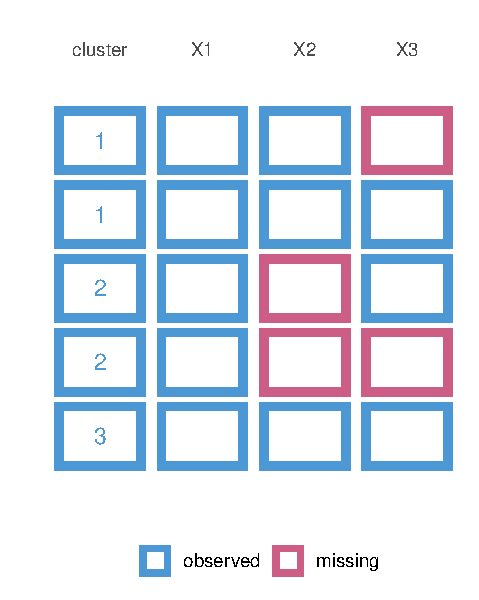
\includegraphics{Manuscript_files/figure-latex/patterns-1} \end{center}

\end{CodeChunk}

\begin{itemize}
\item
  What kinds of missingness are there? ADD: missingness mechanisms here.
  See e.g. \citet{yuce08} and \citet{hox15}.
\item
  Why are standard (ad hoc) missing data methods not well suited?
\item
  What types of multilevel methods are available? General overview of
  approaches, see \citet{audi18} and \citet{grun18}. E.g., imputation of
  study level versus patient-level covariates, and one-stage imputation
  versus two-stage imputation methods.
\item
  Additional difficulty that is addressed in this tutorial: MNAR data.
\end{itemize}

\hypertarget{aim-of-this-paper}{%
\subsection{Aim of this paper}\label{aim-of-this-paper}}

\begin{itemize}
\item
  Provide practical guidelines with code snippets for imputation of
  incomplete multilevel data.
\item
  We focus on the workflow for conditional modeling (not JOMO) in
  \texttt{mice}. Refer to other packages: \texttt{mitml},
  \texttt{miceadds}, \texttt{mdmb}.
\item
  Case study options: \texttt{metamisc::impact} (real IPD on traumatic
  brain injuries, without \texttt{NA}s), \texttt{mice::popularity}
  (simulated data on school kids, with MNAR/MAR mixture). TODO: Check
  example data Gelman.
\item
  Introduce case study and set scope of this tutorial: We're providing
  an overview of implementations. It's up-to the reader to decide which
  strategy suits their data. So we won't go into detail for the
  different methods (and equations). This paper is just a software
  tutorial. We'll keep it practical. -\textgreater{} ADD: some kind of
  help function that suggests a suitable predictor matrix to the user,
  given a certain analysis model.
\end{itemize}

\hypertarget{workflows}{%
\section{Workflows}\label{workflows}}

We'll use the IMPACT data (\texttt{metamisc::impact}) and a MAR/MNAR
version of the \texttt{mice::popmis} data (i.e., a variation on the Hox
(2010) popularity data, where the missingness in the variables is either
missing at random (MAR) or missing not at random (MNAR)).

\hypertarget{case-study-i-impact}{%
\subsection{Case study I: IMPACT}\label{case-study-i-impact}}

\begin{itemize}
\item
  What does the data look like? \texttt{impact} is traumatic brain
  injury data with patients clustered in studies,
  \(n_{\text{participants}} = 11022\) and \(n_{\text{clusters}} = 15\),
  on the following 11 variables:

  \begin{itemize}
  \tightlist
  \item
    \texttt{name} Name of the study,
  \item
    \texttt{type} Type of study (RCT: randomized controlled trial, OBS:
    observational cohort),
  \item
    \texttt{age} Age of the patient,
  \item
    \texttt{motor\_score} Glasgow Coma Scale motor score,
  \item
    \texttt{pupil} Pupillary reactivity,
  \item
    \texttt{ct} Marshall Computerized Tomography classification,
  \item
    \texttt{hypox} Hypoxia (0=no, 1=yes),
  \item
    \texttt{hypots} Hypotension (0=no, 1=yes),
  \item
    \texttt{tsah} Traumatic subarachnoid hemorrhage (0=no, 1=yes),
  \item
    \texttt{edh} Epidural hematoma (0=no, 1=yes),
  \item
    \texttt{mort} 6-month mortality (0=alive, 1=dead).
  \end{itemize}
\end{itemize}

\begin{CodeChunk}
\begin{CodeOutput}
 /\     /\
{  `---'  }
{  O   O  }
==>  V <==  No need for mice. This data set is completely observed.
 \  \|/  /
  `-----'
\end{CodeOutput}


\begin{center}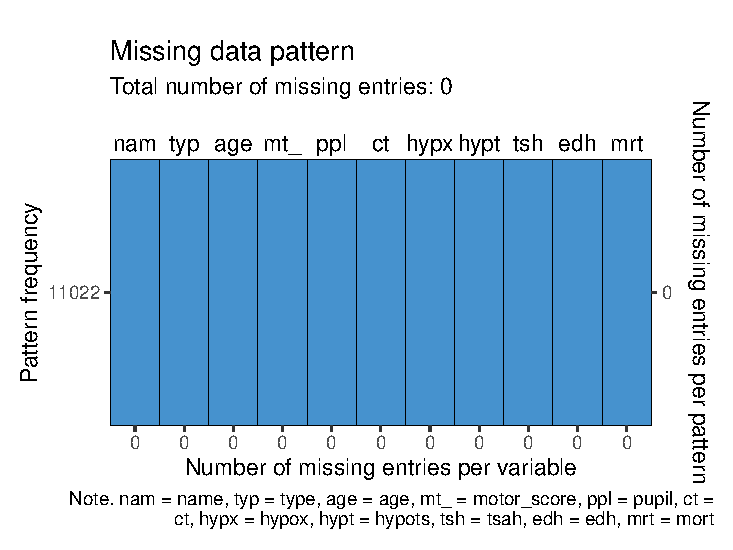
\includegraphics{Manuscript_files/figure-latex/impact-1} \end{center}

\end{CodeChunk}

-\textgreater{} Why are there no missings? According to the
\href{https://cran.r-project.org/web/packages/metamisc/metamisc.pdf}{vignette},
the data is already imputed (Steyerberg et al, 2008).

\hypertarget{case-study-ii-popularity}{%
\subsection{Case Study II: Popularity}\label{case-study-ii-popularity}}

\begin{itemize}
\item
  What does the data look like? \texttt{popNCR} is a simulated dataset
  with pupils clustered in classes, \(n_{\text{participants}} = 2000\),
  \(n_{\text{clusters}} = 100\), on 7 variables:

  \begin{itemize}
  \tightlist
  \item
    \texttt{pupil} Pupil number within class,
  \item
    \texttt{class} Class number,
  \item
    \texttt{extrav} Pupil extraversion,
  \item
    \texttt{sex} Pupil gender,
  \item
    \texttt{texp} Teacher experience (years),
  \item
    \texttt{popular} Pupil popularity,
  \item
    \texttt{popteach} Teacher popularity.
  \end{itemize}
\item
  What are the ICCs? For \texttt{popular} the ICC is 0.33. For
  \texttt{popteach} it is 0.31.
\item
  What does the missingness look like? Induced MAR/MNAR missingness.
  Missing data pattern:
\end{itemize}

\begin{CodeChunk}


\begin{center}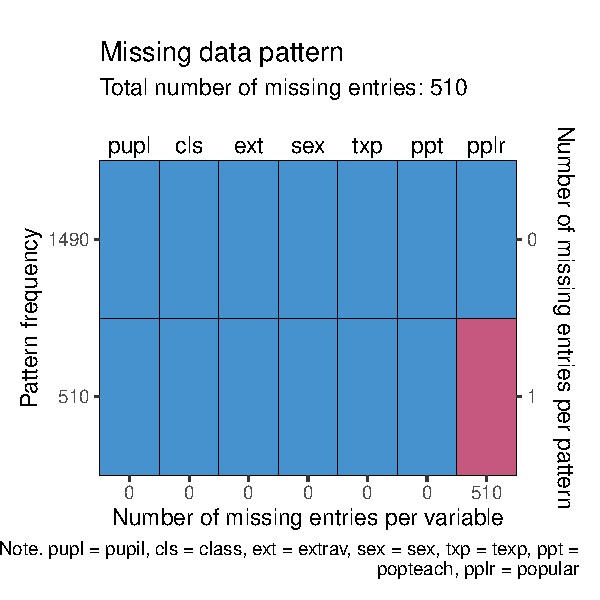
\includegraphics{Manuscript_files/figure-latex/pop_pat-1} \end{center}

\end{CodeChunk}

\begin{itemize}
\item
  Does the missing data of popular depend on popteach? One could for
  example check this by making a histogram of popteach separately for
  the pupils with known popularity and missing popularity. We do see
  that the histogram for the missing popular (TRUE) is further to the
  right than the histogram for observed popular (FALSE). This would
  indicate a right-tailed MAR missingness. In fact this is exactly what
  happens, because we created the missingness in these data ourselves.
  But we can make it observable by examining the relations between the
  missingness in popular and the observed data in popteach.
\item
  Does the missingness in teacher popularity depend on pupil popularity?
  Yes: there is a dependency. The relation seems to be right-tailed.
\end{itemize}

\begin{CodeChunk}


\begin{center}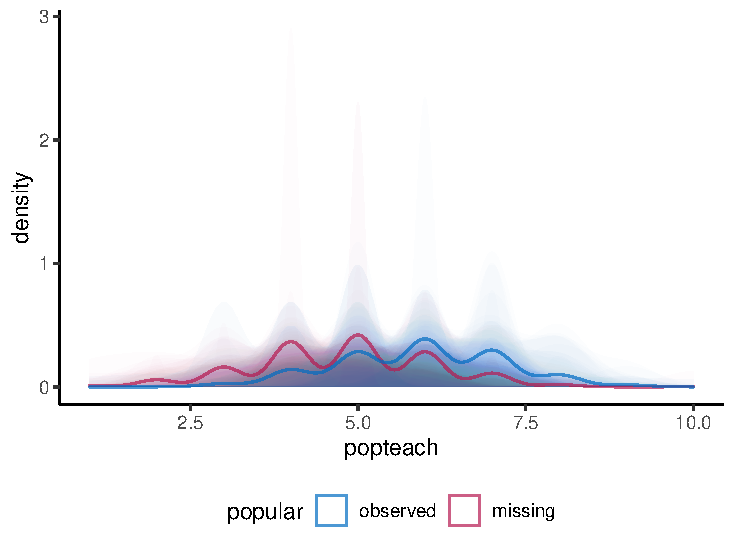
\includegraphics{Manuscript_files/figure-latex/pop_dist-1} \end{center}



\begin{center}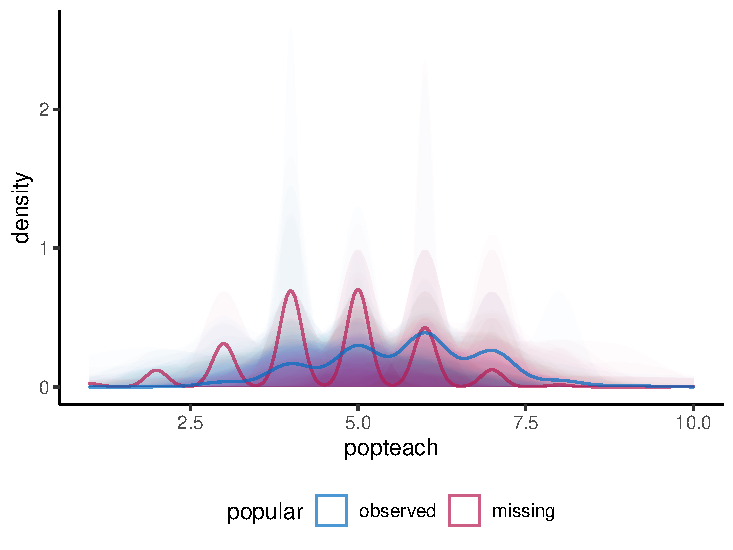
\includegraphics{Manuscript_files/figure-latex/pop_dist-2} \end{center}

\end{CodeChunk}

\hypertarget{modeling-choices}{%
\subsection{Modeling choices}\label{modeling-choices}}

\begin{itemize}
\item
  Which models will we discuss? We'll build the model to grow in
  complexity. The final model is the most complex but also the most
  versatile.
\item
  Note on model complexity: Typically, we should at least use random
  intercepts, but often random slopes as well. Ideally we impute with
  random everything and heteroscedastic errors: most generic method (no
  worry about congeniality, but don't mention the term) -\textgreater{}
  Refer to other papers for background, we'll focus just on the software
  implementation of the situations mentioned there. Sometimes there's
  little reason to assume some variable is affected by heterogeneity.
  -\textgreater{} Refer to Meng, Vincent, and a paper by Grund on
  congeniality and random slopes.
\item
  Step 0: As predictor
\item
  Step 1: Random intercepts
\item
  Step 2: Random slopes
\item
  Step 3: Residuals
\item
  Heckman model for MNAR
\item
  What do the different implementations look like? How to define the
  imputation model(s) in \texttt{mice}?
\end{itemize}

\hypertarget{step-0}{%
\subsection{Step 0}\label{step-0}}

\begin{itemize}
\item
  AKA multilevel imputation for dummies.
\item
  Doesn't work for systematic missingness.
\end{itemize}

\hypertarget{step-1-3}{%
\subsection{Step 1-3}\label{step-1-3}}

\begin{itemize}
\tightlist
\item
  TODO: fill in.
\end{itemize}

\hypertarget{pooling}{%
\subsection{Pooling}\label{pooling}}

\begin{itemize}
\item
  Analysis of scientific interest.
\item
  Pooling using \texttt{mitml}.
\item
  Pooling `regular' parameters vs more `exotic' parameters (SE of
  residual errors, or autocorrelation)
\item
  ADD: export \texttt{mids} objects to other packages like \texttt{lme4}
  or \texttt{coxme}?
\end{itemize}

\hypertarget{discussion}{%
\section{Discussion}\label{discussion}}

\begin{itemize}
\item
  JOMO in \texttt{mice} --\textgreater{} on the side for now
\item
  Additional levels of clustering
\item
  Timeseries: and polynomial relationship in the clustering.
\end{itemize}

\renewcommand\refname{References}
\bibliography{../References/multilevelmice.bib}


\end{document}
